\chapter{Desenvolvimento}\label{chp:desenvolvimento}

Para realização da solução proposta nesse trabalho, é necessário o desenvolvimento de um aplicativo móvel para que o rastreamento de doenças infecciosas ocorra de forma automática. Assim, na Seção \ref{sec:requisitos} são apresentados os requistos funcionais e não funcionais do sistema, junto com a análise de cada um deles. A Seção \ref{sec:modelagem} tem o propósito de apresentar todo o processo de modelagem do sistema, discutindo sobre o racional por trás de cada modelagem e apresentando os diagramas construídos. Na Seção \ref{sec:uiux} são apresentadas as interfaces construídas para o aplicativo. A Seção \ref{sec:implementacao} contém a implementação das interfaces, modelagens e infraestrutura do sistema, utilizando o fluxo de trabalho \textit{GitFlow}.

\section{Levantamento e Análise de Requisitos}\label{sec:requisitos}
O aplicativo deve automatizar todo o ciclo do rastreamento, desde a captura da exposição à uma doença, até a notificação feita à pessoa possivelmente exposta. Com isso, a partir do problema de rastreamento de contatos apresentado no Capítulo \ref{chp:Introducao}, o processo de análise de requisitos foi feito pensando nos possíveis casos de uso do usuário.

Começando pelos requisitos não funcionais, a eficácia da solução depende diretamente do número de usuários que utilizarem o aplicativo. Por conta disso, o aplicativo deve funcionar em diferentes tipos de sistema operacionais de dispositivos móveis, a fim de atingir a maior quantidade de usuários.

Para que esse requisito seja atendido, o aplicativo pode ser desenvolvido especialmente para cada tipo de \Sigla{Sistema Operacional}{SO} ou utilizando um \textit{framework} híbrido, em que a partir da mesma base de código é possível construir os arquivos para cada SO.

Levando em consideração o tempo de desenvolvimento do aplicativo e o número de pessoas envolvidas, a utilização de um \textit{framework} híbrido é a melhor forma para atingir o maior número de usuários.

Além disso, como o aplicativo armazena os dados de localizações dos usuários, ele deve se preocupar em garantir a segurança dos mesmos. Essa segurança será garantida a partir da utilização de criptografia. Ela será aplicada aos dados em trânsito e em repouso, ou seja, tanto durante a comunicação entre cliente e servidor quanto no armazenamento no BD.

Ainda relacionado à segurança, a fim de preservar a privacidade das pessoas que utilizarem o aplicativo, a aplicação ou os usuários não devem ser capazes de descobrir quem possivelmente expôs outras pessoas a alguma doença. Isso significa que quando um usuário receber uma notificação de exposição, ele não será capaz de identificar quem foi, nem o local que isso ocorreu.

Para isso, o aplicativo não terá a inserção de nenhum dado pessoal, ou seja, a autenticação será feita de forma anônima, onde cada usuário será representado por uma cadeia de caracteres aleatórios.

Por último, toda localização terá prazo de validade de 14 dias. Isso significa que todo local visitado pelo usuário será armazenado apenas durante esse prazo. Como a solução do problema é a automação do rastreamento de contatos, localizações mais antigas do que esses dias não são necessárias, já que o período de transmissão do vírus haveria terminado.

A partir do que foi explicado nos parágrafos anteriores, foram levantados 3 requisitos não funcionais. Esses requisitos são:

\begin{enumerate}
  \item Compatibilidade multiplataforma;
  \item Garantia de privacidade e segurança dos dados;
  \item Exclusão de localizações antigas;
\end{enumerate}

Como o aplicativo usará um \textit{framework} multiplataforma para atender os requisitos não funcionais citados anteriormente, essa escolha trás um malefício: recursos nativos de cada dispositivo, como por exemplo o \textit{Bluetooth}, não possuem o mesmo suporte caso fosse uma codificação utilizando uma linguagem nativa.

Levando isso em consideração, os contatos que eventualmente ocorrerem entre diferentes usuários do aplicativo podem ser rastreados a partir de duas principais formas: 

\begin{itemize}
  \item Armazenamento dos locais visitados pelos usuários utilizando um sistema de \textit{check-in}, onde o usuário fará a inserção do local visitado utilizando um sistema de busca;
  \item Armazenamento dos contatos que foram efetuados utilizando o \textit{Bluetooth}. O dispositivo detectará os sinais transmitidos ao seu redor, e fará a persistencia desses contatos;
\end{itemize}

Ambas soluções solucionam o problema de formas distintas, porém, levando em consideração o requisito de compatibilidade multiplataforma e do baixo acesso à recursos nativos pelos \textit{frameworks}, a solução utilizada neste trabalho será a partir do sistema de \textit{check-in}.

Com isso, os usuários necessitam de um buscador para encontrar os locais que foram visitados. Esse buscador deve estar relacionado a um extenso BD para que a maioria dos locais inseridos pelos usuários sejam encontrados. Por conta disso, um BD externo deve ser utilizado, já que a criação de uma nova não traria a experiência esperada para o usuário.

Depois que a busca foi feita, o usuário deve ser capaz de salvar o local encontrado. O salvamento deve ser feito em um BD remoto, para que a rotina de checagem do rastreamento de contatos seja feita no servidor. Com isso, o dispositivo móvel do usuário não precisará de conectividade com a \textit{internet}, nem que o aplicativo rode em segundo plano durante a execução da rotina, evitando o consumo desnecessário de bateria do dispositivo.

Se um usuário for infectado por uma doença, ele deve ser capaz de declarar no aplicativo que está infectado. A partir disso, a rotina de rastreamento de contatos deve ser capaz de relacionar os locais do usuário infectado com os usuários comuns, procurando por algum possível contato que possa ter ocorrido.

O usuário deve receber notificações caso o mesmo tenha tido algum possível contato com outras pessoas que utilizam o aplicativo e estavam infectadas. Essa notificação deve ser enviada de forma automática e sem a necessidade de intervenção humana, para que o problema seja resolvido de forma automática de ponta a ponta.

A partir de toda análise acima, foram levantados 4 requisitos funcionais, que são:

\begin{enumerate}
  \item Buscar localizações;
  \item Salvar localizações;
  \item Declarar caso de infecção confirmado;
  \item Enviar notificação de exposição;
\end{enumerate}

\section{Modelagem}\label{sec:modelagem}
% https://proandroiddev.com/clean-architecture-data-flow-dependency-rule-615ffdd79e29
% https://github.com/android10/Android-CleanArchitecture/issues/136
% https://blog.cleancoder.com/uncle-bob/2012/08/13/the-clean-architecture.html
% https://resocoder.com/2019/08/27/flutter-tdd-clean-architecture-course-1-explanation-project-structure/

O processo de modelagem foi feito desde os aspectos mais abstratos do sistema, utilizando os diagramas de componentes e de pacotes, até os mais específicos, utilizando os diagrama de sequência e de atividades.

Para melhor apresentação e discussão de cada uma das modelagens, elas estão dividas nas subseções abaixo.

\subsection{Modelagem dos componentes do sistema}
% Diagrama de componentes
Esta Seção conterá a modelagem do diagrama de componentes, que será responsável por representar o funcionamento e a relação dos diferentes componentes do sistema, ou seja, a relação entre o aplicativo móvel utilizado pelo usuário, com o BD, \textit{backend} e o sistema de mensageria.

\subsection{Modelagem da arquitetura do \textit{software}}
% Modelagem mais abstrata da arquitetura: pacotes
% Modelagem mais específica: classes
Como explicado na Seção \ref{sec:clean}, o aplicativo desenvolvido neste trabalho utiliza os princípios da arquitetura limpa. Por conta disso, a base da arquitetura do \textit{software} é a \Figura{fig:clean1}.

Antes de começar a diagramação, é importante entender a diferença entre dependência e fluxo de dados do aplicativo, porque essa diferença é crucial para que a modelagem não quebre nenhuma das regras da arquitetura limpa.

A dependência do código acontece no tempo de compilação, ou seja, só há dependência entre os componentes se houver uma referência direta para outro componente.

Por exemplo, imagine que em uma das classes da camada \textit{Application Business Rules} do aplicativo possua um caso de uso que em sua implementação exista uma chamada para um método de uma classe presente na camada \textit{Interface Adapters}. Nesse exemplo, o caso de uso possuiria dependência com a camada \textit{Interface Adapters}, e estaria ferindo a regra de dependência, já que essa é uma camada externa em relação à \textit{Application Business Rules}.

Já o fluxo de dados seria equivalente ao fluxo de chamadas dentro do código, que não acontece no tempo de compilação, e sim no de execução. Pode parecer contraditório, mas a dependência nem sempre reflete o fluxo de dados do código.

Utilizando o mesmo exemplo anterior, é possível fazer com que o caso de uso não dependa da camada \textit{Interface Adapters}, mas ainda consiga atingir o mesmo comportamento esperado. Para que isso aconteça, uma interface deve ser criada na camada \textit{Application Business Rules}, e ela conterá as assinaturas dos métodos que o caso de uso necessita. Na camada \textit{Interface Adapters}, uma classe implementará os métodos definidos na interface através do relacionamento de herança.

Dessa maneira, através do \textit{Dependency Inversion Principle}, explicado na subseção \ref{sec:D}, a dependência existirá da camada \textit{Interface Adapters} para a camada \textit{Application Business Rules} por conta da herança, mas no fluxo de chamadas em tempo de execução, será da \textit{Application Business Rules} para a camada \textit{Interface Adapters}.

Com a diferença entre dependência e fluxo de dados compreendida, toda modelagem da arquitetura do sistema deve fazer com que nenhuma camada interna dependa de uma mais externa à ela. Para isso, todas as fronteiras das camadas haverão interfaces para possibilitar a comunicação sem que a regra de dependência seja ferida.

Como o aplicativo fará chamadas para componentes de persistência de dados, utilizando APIs para busca de locais e um BD remoto para o armazenamento, essas chamadas serão realizadas utilizado o padrão de repositório. A partir disso, o fluxo dos dados entre os componentes do sistema serão nessa ordem:

\begin{enumerate}
  \item \textit{View} faz chamadas dos métodos da \textit{View Model};
  \item \textit{View Model} executa o caso de uso;
  \item Caso de uso combina os dados dos repositórios das entidades;
  \item Cada repositório retorna os dados dos \textit{Data Sources};
  \item Os dados voltam para a \textit{View} e são mostrados ao usuário;
\end{enumerate}

A partir dessa ordem, a adaptação da \Figura{fig:clean1} com o padrão de repositório e da diferença entre dependência e fluxo de dados é feita na \Figura{fig:cleanadapt}.

\begin{figure}[!htb]
  \centering
  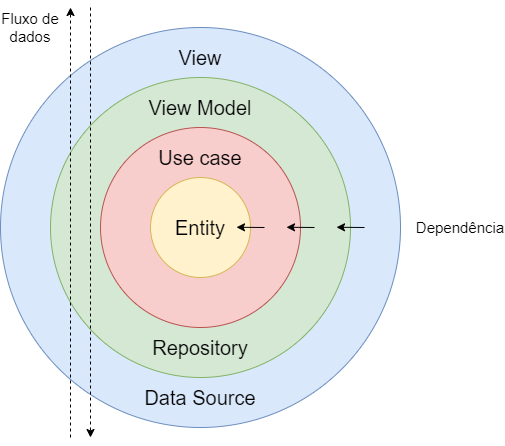
\includegraphics[scale=0.6]{clean-adapt.png}
  \caption{Diferença entre dependência e fluxo de dados.}
  \label{fig:cleanadapt}
\end{figure}

Note que as dependências estão sempre apontando para o interior. Levando em consideração a explicação de como as fronteiras das camadas são passadas através da inversão de dependências, o diagrama de pacotes da \Figura{fig:package} possui a modelagem mais abstrata e de maior alto nível da arquitetura do aplicativo. 

% imagem do diagrama de pacotes 
\begin{figure}[!htb]
  \centering
  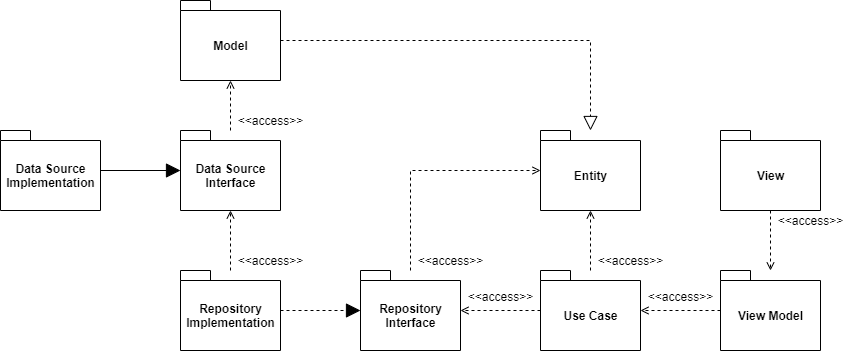
\includegraphics[scale=0.7]{Diagrama de pacotes.png}
  \caption{Diagrama de pacotes do aplicativo.}
  \label{fig:package}
\end{figure}

Para que a associação do diagrama da \Figura{fig:package} com as camadas e regras de dependência da \Figura{fig:clean1} sejam melhor visualizados, a \Figura{fig:package2} representa as camadas da arquitetura limpa, com as mesmas colorações, por cima do diagrama de pacotes.

\begin{figure}[!htb]
  \centering
  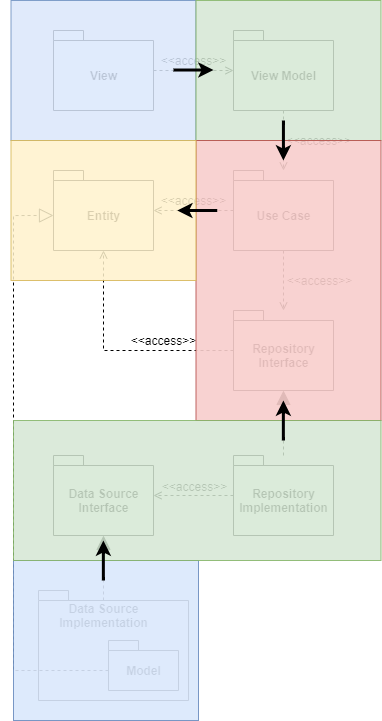
\includegraphics[scale=0.7]{package-adapt.png}
  \caption{Diagrama de pacotes com as colorações das camadas da arquitetura limpa.}
  \label{fig:package2}
\end{figure}

\subsection{Modelagem dos casos de uso}
% Modelagem geral: casos de uso
% Modelagem de cada caso de uso: atividade e sequência
Os casos de uso do sistema são herdados do levantamento de requisitos. Por conta disso, a partir do que foi discutido na Seção \ref{sec:requisitos}, o diagrama de casos de uso está representado pela \Figura{fig:usecasesdiagram}.

\begin{figure}[!htb]
  \centering
  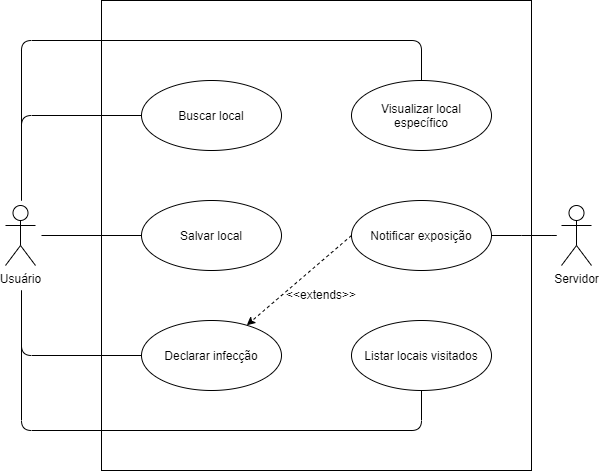
\includegraphics[scale=0.7]{Diagrama de casos de uso.png}
  \caption{Diagrama de casos de uso.}
  \label{fig:usecasesdiagram}
\end{figure}

Cada caso de uso da \Figura{fig:usecasesdiagram} é uma funcionalidade. Para cada uma delas serão modelados os diagramas de atividade e de sequência.

A modelagem do diagrama de atividades possuirá o objetivo de entender o processo e os comportamentos de cada funcionalidade. Já o diagrama de sequência descreverá como e em que ordem um grupo de objetos trocam mensagens entre si, ou seja, a forma que eles funcionam em conjunto.

\subsection{Modelagem de dados}
% https://www.youtube.com/watch?v=35RlydUf6xo
% https://medium.com/flutterdevs/firebase-data-modeling-tips-2fc61724743a
% https://fireship.io/courses/firestore-data-modeling/

Esta Seção conterá as informações e discussões sobre a modelagem de dados do BD \textit{Firestore}, com o objetivo de entender o motivo dos dados estarem dispostos da maneira que foram modelados.

\section{Interfaces de usuário do aplicativo}\label{sec:uiux}
Esta Seção conterá os \textit{layouts} das telas construídas no aplicativo móvel.

\section{Implementação}\label{sec:implementacao}
Esta Seção conterá as informações sobre como a interface de usuário, as modelagens e a infraestrutura do sistema foram construídas e configuradas, contendo exemplos de trechos da implementação.

Além disso, também mostrará como o projeto foi gerenciado no \textit{GitHub}, mostrando o quadro \textit{Kanban} utilizado, com a criação das \textit{issues} - que representam as tarefas que deveriam ser concluídas - e mostrando um exemplo de funcionamento prático do fluxo de trabalho \textit{GitFlow}.